% !TeX spellcheck = ru_RU-Russian
\documentclass[11pt]{article}
\usepackage{ucs} 
\usepackage[utf8x]{inputenc} % Включаем поддержку UTF8  
\usepackage[russian]{babel}  % Включаем пакет для поддержки русского языка 
\usepackage {mathtext}
\usepackage{mathrsfs, amsmath, amssymb}
\usepackage{graphicx}
\usepackage{listings}
\usepackage{hyperref}
\usepackage{revsymb}
\usepackage{listings}
\usepackage{longtable}
\usepackage{float}
\lstset{language=[90]Fortran,
	basicstyle=\ttfamily,
	keywordstyle=\color{red},
	commentstyle=\color{green},
	morecomment=[l]{!\ }% Comment only with space after !
}
\hypersetup{
	colorlinks=true,
	linkcolor=blue,
	filecolor=magenta,      
	urlcolor=cyan,
}
\urlstyle{same}
\DeclareGraphicsExtensions{.pdf,.png,.jpg,.jpeg}

\graphicspath{{pictures/}}
\title{\textbf{Практическое занятие 3.1  \\ -- \\ 
		Применение диагностических методов, подбор технических средств и их параметров для реализации выбранного метода в зависимости от показаний}}
\author{И.А.Юхновский}
\date{июнь 2021}

\begin{document}
	
	\maketitle
	\thispagestyle{empty}
	\section*{Аннотация}
	На примере комплексной лучевой диагностики остеонекрозов у дезоморфинзависимых пациентов закрепляется на практике тема лекции 3.1 "Биофизические и биохимические механизмы действия диагностических методов и основные группы методов диагностики, ориентированных на изучение различных проявлений жизнедеятельности организма" дисциплины "Технические методы диагностических исследований и лечебных воздействий" по направлению 12.03.04 "Биотехнические системы и технологии".
	
		\tableofcontents{}
	
	\section{Введение}
	Дезоморфин – наркотик,	изготовляемый кустарным способом посредством экстрагирования из кодеиносодержащих препаратов, которые можно было свободно приобрести в аптечной сети на территории РФ вплоть до 01.06.2012 года. 
	 
	Данный наркотик впервые был синтезирован в 1933 году в США. Являясь более сильным анальгетиком, чем морфин, этот препарат из-за быстрого возникновения наркозависимости не нашел должного медицинского  применения. Раствор дезоморфина, приготовленный в кустарных условиях с использованием различных ингредиентов (кодеин,	бензин, сода, йод, ацетон, красный фосфор и т.д.), загрязненный промежуточными продуктами синтеза, является нестабильным веществом, поэтому незамедлительно употребляется наркоманами, без возможности его транспортировки  ~\cite{kataev}.

	Несмотря на введенный с 01 июня 2012 г. запрет безрецептурной продажи кодеинсодержащих препаратов на территории РФ, в ведущие лечебные заведения страны ежедневно обращаются пациенты в прошлом или по сей день употребляющие наркотики на основе дезоморфина ~\cite{rejr}. 
	
	Входящий в состав наркотика красный фосфор вызывает развитие атипичных остеонекрозов костей лицевого черепа при внутривенном введении дезоморфина  ~\cite{babkova}. Данный вид остеонекрозов по клинической картине схож с ранее описанными	в литературе случаями фосфорных остеомиелитов челюстей, связанных с фосфорным производством спичек  в конце 19 века ~\cite{basin}. 
	
	\section{Клиническая картина}
	Остеонекрозы  у  лиц  с  наркотической  зависимостью от дезоморфина и первитина представляют собой тяжелые  гнойно-некротические  заболевания  костей лицевого черепа ~\cite{rsj_1,rsj_2,rsj_3,rsj_4,rsj_5,rsj_6,rsj_7,rsj_8,rsj_9,rsj_10,rsj_11,rsj_12,rsj_13,rsj_14,rsj_15}
	
	По данным клинической картины , у всех пациентов отмечали: обнажение костной ткани, развившееся после удаления зуба и сохраняющееся более 8 нед, упорное  гнойное  отделяемое  с  ихорозным  запахом; прогрессирование рецессии десны; отсутствие видимых элементов размягчения кости и грануляционной ткани; повышенная плотность костной ткани; отсутствие зон демаркации и увеличение сроков формирования секвестров; наличие патологических переломов челюстей; массивные периостальные разрастания новообразованной костной ткани в местах присоединения надкостницы к костям лицевого черепа.~\cite{rsj}
	
	\begin{figure}[H]
		\centering
		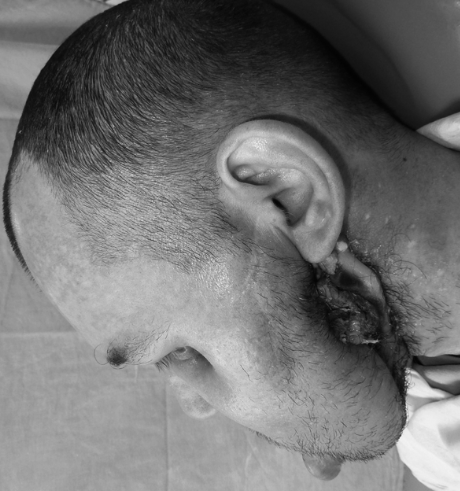
\includegraphics[width=\textwidth]{ris_1}
		\caption{Пациент  П., 44 года. Обширные оростомы в околоушно-жевательных областях, парез лицевого нерва слева ~\cite{rsj}.}
		\label{fig:ris_1}
	\end{figure}

	\begin{figure}[H]
	\centering
	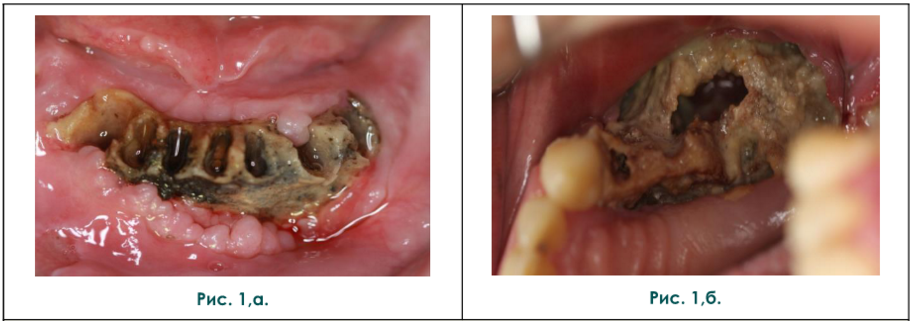
\includegraphics[width=\textwidth]{ris_2}
	\caption{Фотографии внешнего вида нижней (а) и верхней (б) челюстей при стоматологическом 
		осмотре. ~\cite{rejr}.}
	\label{fig:ris_2}
	\end{figure}
	
	\begin{figure}[H]
	\centering
	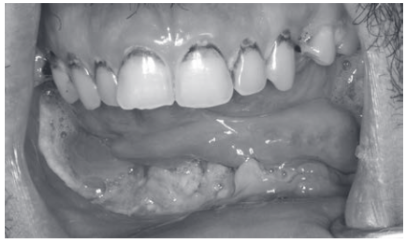
\includegraphics[width=\textwidth]{st1}
	\caption{Обнажение альвеолярной части нижней челюсти, гнойное отделяемое. ~\cite{st}.}
	\label{fig:st1}
	\end{figure}

	\begin{figure}[H]
		\centering
		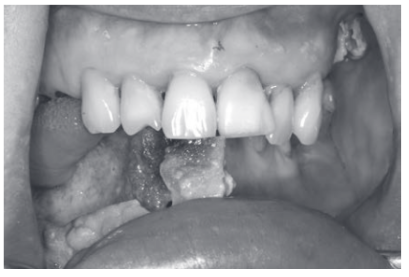
\includegraphics[width=\textwidth]{st2}
		\caption{Патологический перелом нижней челюсти, обнажение костной ткани верхней и нижней челюсти. ~\cite{st}.}
		\label{fig:st2}
	\end{figure}

	\begin{figure}[H]
	\centering
	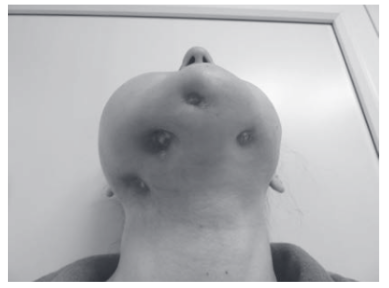
\includegraphics[width=\textwidth]{st3}
	\caption{Внутренние свищевые ходы с гнойным отделяемым без выбухающих грануляций. ~\cite{st}.}
	\label{fig:st3}
	\end{figure}

	\begin{figure}[H]
	\centering
	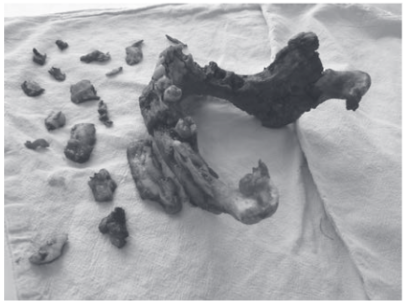
\includegraphics[width=\textwidth]{st4}
	\caption{Тотальный некроз нижней челюсти (макропрепарат). ~\cite{st}.}
	\label{fig:st4}
	\end{figure}


	\begin{figure}[H]
		\centering
		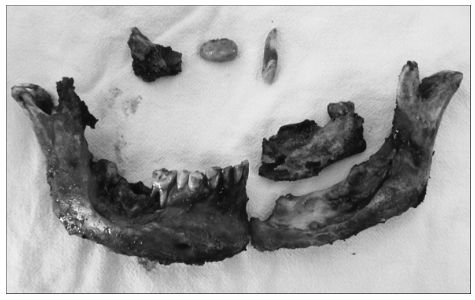
\includegraphics[width=\textwidth]{nch}
		\caption{Макропрепарат нижней челюсти. ~\cite{rsj}.}
		\label{fig:nch}
	\end{figure}
	
	
	\section{Цель практического занятия}
	Определение диагностической эффективности методов лучевой диагностики  (ортопантомография, рентгенография черепа, МСКТ, КЛКТ, радионуклидная диагностика) в оценке остеонекрозов у дезоморфинзависимых пациентов на 
	до- и послеоперационных этапах лечения.
		
	\section{Материалы и методы}
	В практической работе приведены иллюстрации из ~\cite{rsj, rejr}. 
	
	Диагностика остеонекрозов и последующее планирование оперативного вмешательства	в настоящее время основаны на результатах	применения комплекса методов лучевых исследований:
	\begin{itemize} 
		\item ОПТГ - ортопантомография;
		\item рентгенография;
		\item МСКТ - мультиспиральная компьютерная томография;
		\item КЛКТ - конусно-лучевая компьютерная томография;
		\item остеосцинтиграфия.
	\end{itemize} 
	
	\section{ОПТГ}
	Ортопантомография (ОПТГ) можно применять на 2 этапах лечения: 
	\begin{itemize} 

	\item На этапе первичной консультации ОПТГ позволяет оценить общее состояние всей зубочелюстной системы (костной ткани, зубов, периодонта, пародонта), примерную распространенность остеонекротического процесса, дает характеристику лункам удаленных зубов, позволяет определить наличие, характер, локализацию  перелома, зон остеосклеротического из	менения костной структуры, секвестрации	костной ткани, периостальной реакции. 
	
	\item На послеоперационном этапе лечения данной группы пациентов ОПТГ позволяет оценить качество и 	полноту проведенного оперативного вмешательства, состояние установленных эндопротезов, наличие инородных тел (костные фрагменты, части эндопротезов). 
	
	\end{itemize} 

	\begin{figure}[H]
	\centering
	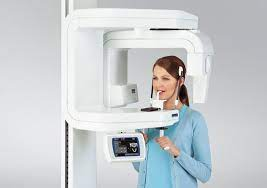
\includegraphics[width=\textwidth]{optg_1}
	\caption{Пример использования ОПТГ}
	\label{fig:optg_1}
	\end{figure}

	\begin{figure}[H]
	\centering
	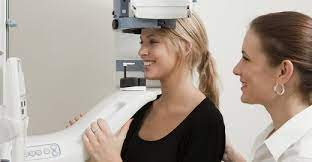
\includegraphics[width=\textwidth]{optg_2}
	\caption{Пример использования ОПТГ}
	\label{fig:optg_2}
	\end{figure}

	\begin{figure}[H]
	\centering
	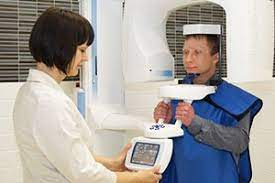
\includegraphics[width=\textwidth]{optg_3}
	\caption{Пример использования ОПТГ}
	\label{fig:optg_3}
	\end{figure}

	\begin{figure}[H]
	\centering
	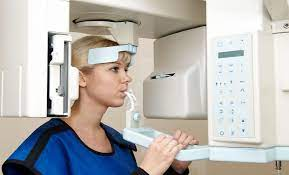
\includegraphics[width=\textwidth]{optg_4}
	\caption{Пример использования ОПТГ}
	\label{fig:optg_4}
	\end{figure}

	ОПТГ является доступным методом диагностики, однако имеет ряд недостатков: 
	\begin{itemize} 
	\item проекционные искажения; 
	\item дополнительные тени (эффект суперпозиции); 
	\item плохая визуализация фронтальной группы зубов, верхней челюсти,верхнечелюстных синусов. 
	\end{itemize} 
	
	\begin{figure}[H]
	\centering
	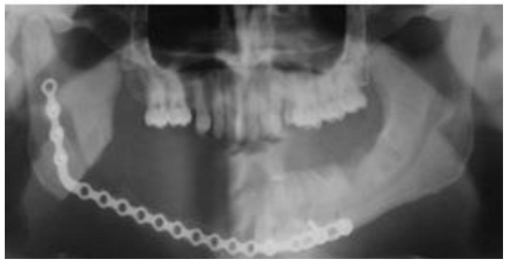
\includegraphics[width=\textwidth]{optg_5}
	\caption{Ортопантомограмма - определяется последовательный дефект тела нижней челюсти справа до уровня угла. В зоне дефекта визуализируется установленный имплантат в виде перфорированной металлической пластины. Пластина анатомически достаточно точно повторяет ход нижней челюсти ~\cite{rejr}. }
	\label{fig:optg_5}
	\end{figure}

	\begin{figure}[H]
	\centering
	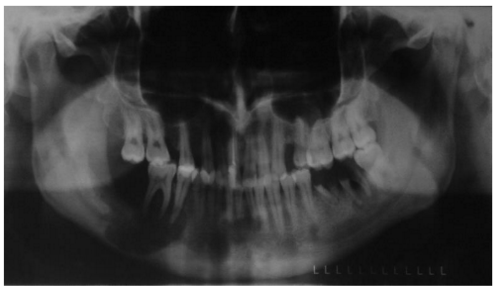
\includegraphics[width=\textwidth]{optg_6}
	\caption{Ортопантомограмма - Определяется очаг деструкции костной ткани в области зубов 3.2-4.6, отсутствующих зубов 4.7, 4.8 с вовлечением канала нижнечелюстного нерва справа. Неполная вторичная адентия: отсутствуют зубы 1.4, 1.8, 2.4, 4.7, 4.8. Определяются остаточные корни зубов 3.6, 3.7. Отмечается остеосклероз в области угла и ветви нижней	челюсти справа ~\cite{rejr}. }
	\label{fig:optg_6}
	\end{figure}

	\begin{figure}[H]
	\centering
	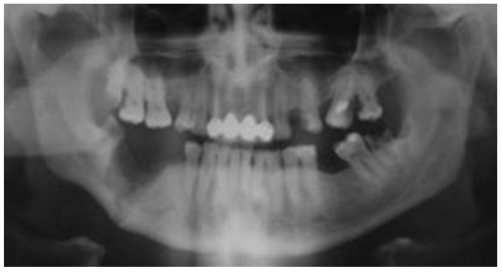
\includegraphics[width=\textwidth]{optg_7}
	\caption{Ортопантомограмма - Определяется очаг деструкции костной ткани в области отсутствующих зубов 4.6-4.7, с вовлечением канала нижнечелюстного нерва справа. Неполная вторичная адентия: отсутствуют зубы 1.5, 1.8, 2.4, 2.8, 3.6, 4.5, 4.6, 4.7.	Коронковые части зубов 1.8, 3.8 разрушены. Отмечается остеосклероз в области угла и ветви, тела нижней челюсти справа, вокруг очага деструкции. Визуализируется линия перелома тела нижней челюсти справа в 
		области 4.6, 4.7. без выраженного смещения отломков ~\cite{rejr}. }
	\label{fig:optg_7}
\end{figure}

	\begin{figure}[H]
	\centering
	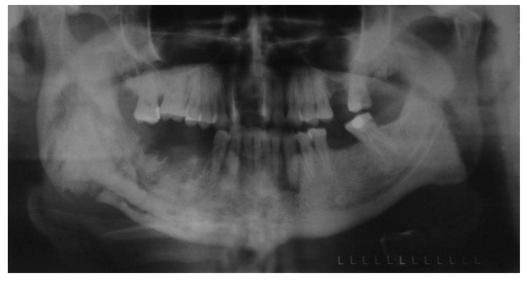
\includegraphics[width=\textwidth]{optg_8}
	\caption{Ортопантомограмма - Определяется очаг деструкции костной ткани от зуба 3.3 до уровня верхней трети ветви нижней челюсти справа, с вовлечением канала нижнечелюстного нерва справа. Неполная вторичная адентия: отсутствуют 
		зубы 1.1, 1.8, 2.6, 2.8, 3.6, 3.8, 4.5, 4.6, 4.7, 4.8. Отмечается секвестрация костной ткани в области ветви, угла, тела нижней челюсти справа, очаги остеосклероза в области ветви, угла, тела нижней челюсти справа, вокруг 
		очага деструкции. В проекции угла, тела нижней челюсти справа визуализируются периостальные наслоения слоистого типа с четкими, местами прерывистыми контурами.  ~\cite{rejr}. }
	\label{fig:optg_8}
	\end{figure}

	\begin{figure}[H]
	\centering
	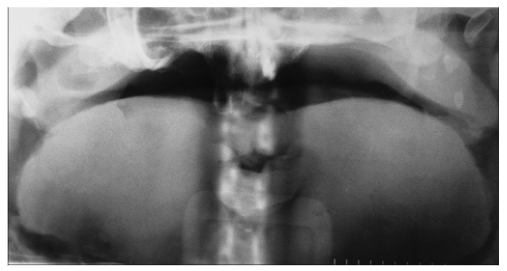
\includegraphics[width=\textwidth]{optg_10}
	\caption{Ортопантомограмма пациента  К., 33 года, после удаления всей нижней и верхней челюсти с обеих сторон, резекции тела скуловой кости с обеих сторон.
	 }
	\label{fig:optg_10}
\end{figure}
	
	Ортопантомография требует обязательного дополнения другими более информативными методами лучевой диагностики (МСКТ, КЛКТ) ~\cite{80-157-1-SM}. 
		
	Иллюстрации выше были сделаны на «ORTHOPANTOGRAPH OP 100»
	
	\begin{figure}[H]
		\centering
		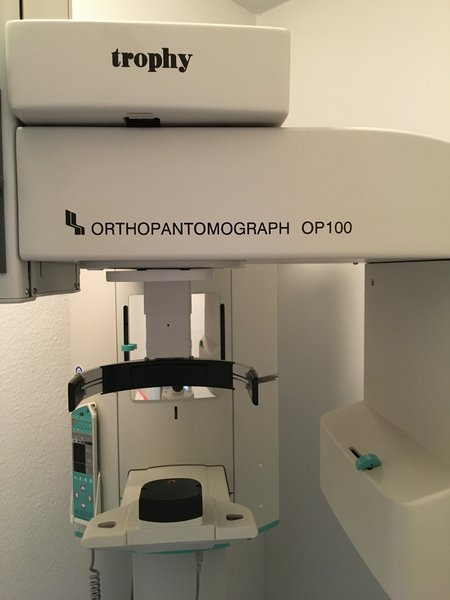
\includegraphics[width=\textwidth]{optg_9}
		\caption{ORTHOPANTOGRAPH OP 100 - внешний вид. }
		\label{fig:optg_9}
	\end{figure}

	Управление и обработка данных осуществляется платой контроллера и встроенным компьютером устройства:
	
	\begin{figure}[H]
		\centering
		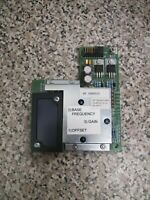
\includegraphics[]{op100_1}
		\caption{ORTHOPANTOGRAPH OP 100 - контроллер. }
		\label{fig:opt100_1}
	\end{figure}

	\begin{figure}[H]
	\centering
	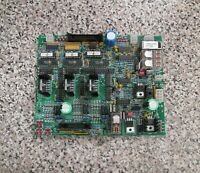
\includegraphics[]{op100_2}
	\caption{ORTHOPANTOGRAPH OP 100 - материнская плата. }
	\label{fig:opt100_2}
	\end{figure}

	Устройство прибора и инструкцию по эксплуатации можно прочитать в  ~\cite{op100}
	\section{Рентгенография}
	Рентгенография  черепа («Silhouette HF» General Electric Medical Systems) проводились всем пациентам (n=85; 100\%) на до- и послеоперационном этапах в стандартной укладке ~\cite{rejr} совместно с ортопантомографией.
	
	\begin{figure}[H]
		\centering
		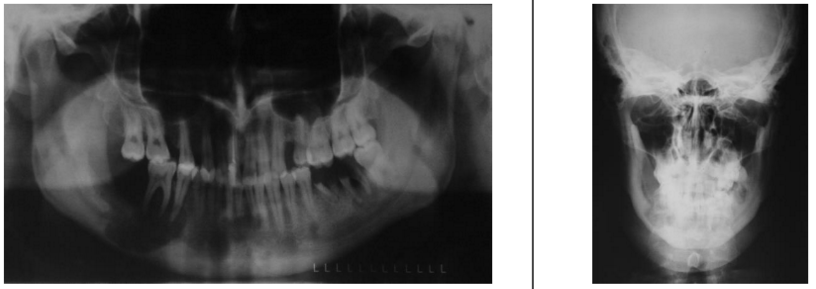
\includegraphics[width=\textwidth]{r1}
		\caption{Ортопантограмма слева и рентгенограмма черепа в прямой проекции справа }
		\label{fig:r1}
	\end{figure}

	\begin{figure}[H]
	\centering
	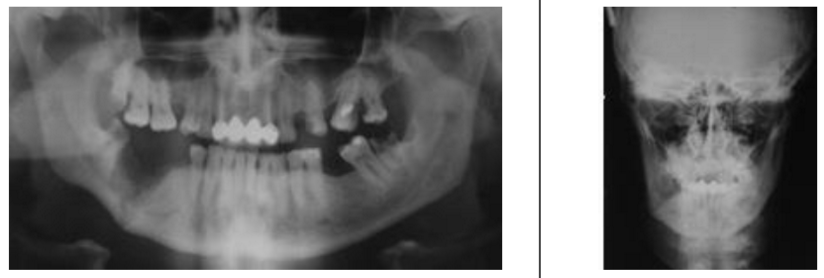
\includegraphics[width=\textwidth]{r2}
	\caption{Ортопантограмма слева и рентгенограмма черепа в прямой проекции справа }
	\label{fig:r2}
	\end{figure}

	\begin{figure}[H]
	\centering
	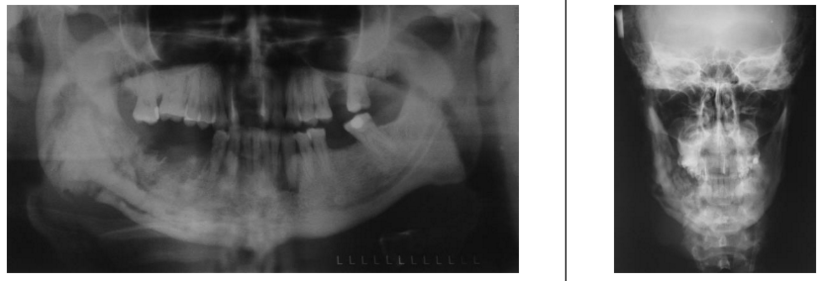
\includegraphics[width=\textwidth]{r3}
	\caption{Ортопантограмма слева и рентгенограмма черепа в прямой проекции справа }
	\label{fig:r3}
	\end{figure}

	Внешний вид установки представлен ниже:
	\begin{figure}[H]
		\centering
		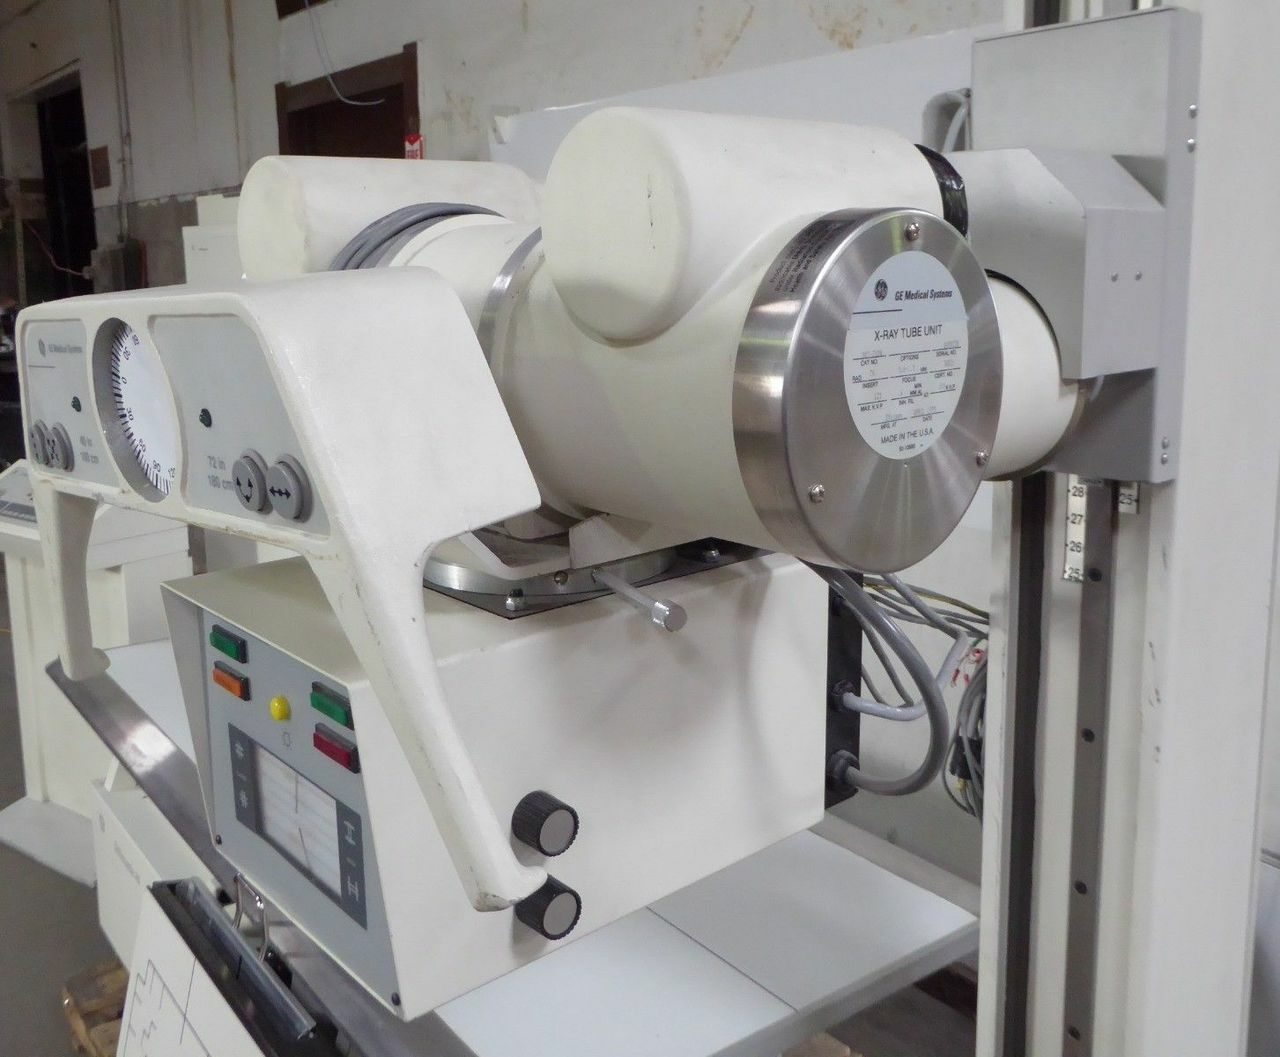
\includegraphics[width=\textwidth]{hf}
		\caption{«Silhouette HF» General Electric Medical Systems}
		\label{fig:hf}
	\end{figure}

	\begin{figure}[H]
		\centering
		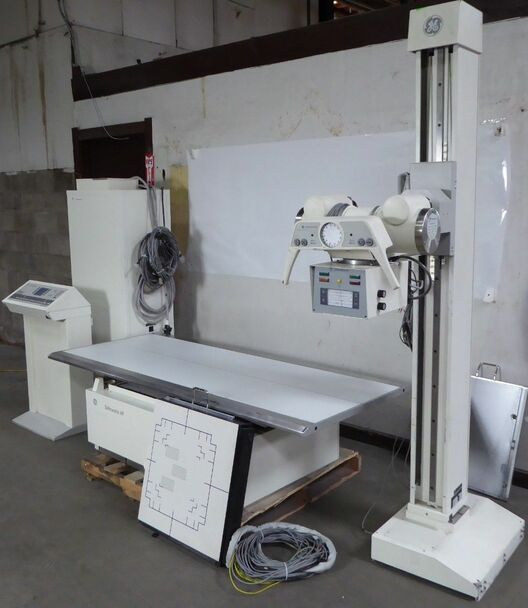
\includegraphics[width=\textwidth]{hf1}
		\caption{«Silhouette HF» General Electric Medical Systems}
		\label{fig:hf1}
	\end{figure}

	\begin{figure}[H]
	\centering
	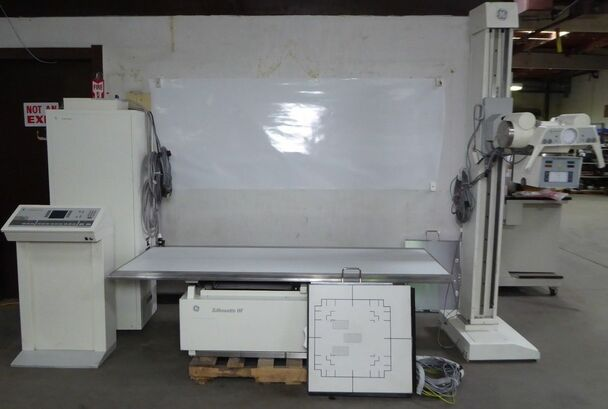
\includegraphics[width=\textwidth]{hf2}
	\caption{«Silhouette HF» General Electric Medical Systems}
	\label{fig:hf2}
	\end{figure}
		
	\begin{figure}[H]
	\centering
	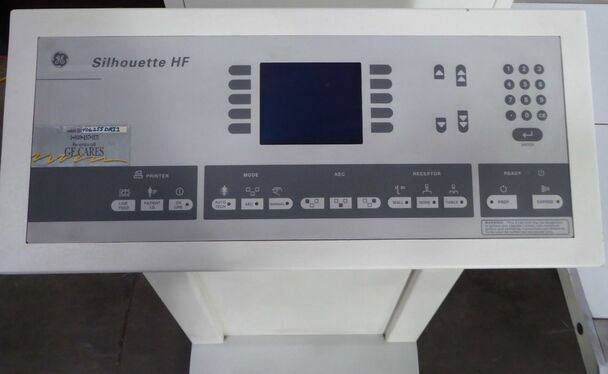
\includegraphics[width=\textwidth]{hf3}
	\caption{«Silhouette HF» General Electric Medical Systems}
	\label{fig:hf3}
	\end{figure}

По данным ортопантомографии и рентгенографии черепа получалось выявить уменьшение размера челюстей за счет наличия выраженного очага остеонекроза (n=54, 63,5\%), у 14 пациентов (16,5\%) значительного изменения размеров челюстей выявлено не было. В 20\% (n=17) случаев определялось увеличение размера нижней челюсти за счет слоистого периостита. Однако определить точные размеры, толщину альвеолярного и небного отростков верхней челюсти, размеры нижней челюсти, структуры и плотности костей челюстно-лицевой области, состояния верхнечелюстных синусов по данным проведенных традиционных рентгенологических методик оказывается невозможным в силу ограниченности этих методов ~\cite{rejr}. 

	\section{ МСКТ - мультиспиральная компьютерная томография}
	В отличие от традиционных рентгенологических методик МСКТ и КЛКТ позволили точно оценить локализацию очагов остеонекроза. 
	Методы позволили оценить изменения	структуры костной ткани челюстно-лицевой области: чередование зон остеосклероза с зонами остеопороза, так называемая картина «мыльной пены» у 24 пациентов (28\%). Очаги остеонекроза по данным МСКТ (КЛКТ) имели неправильную форму, сливающийся характер. Отмечалось отсутствие четкой демаркационной зоны. По  данным  МСКТ  секвестры   были выявлены  у  35  пациентов (41\%), имели в ряде случаев губчатый, кортикальный, смешанный характер. Среди этой группы пациентов свищевые ходы в мягких тканях определялись у 18	пациентов (51,5\%), при этом часть секвестров	относилась к пенетрирующему типу (n=6, 33\%).
	
	 
	МСКТ (КЛКТ) позволили более точно оценить характер и локализацию периостальной реакции, в том числе в области фронтальных отделов челюстей, верхнечелюстных синусов, что 	было невозможно при применении традиционных рентгенологических методик. По данным МСКТ (КЛКТ) явления периостита выявлены у 50 пациентов (59\%). В 23 случаях (46\%) определялся выраженный слоистый характер периостальных наслоений, преимущественно в области нижней челюсти, которые со всех сторон	охватывали кость по типу «муфты».
	
	Данные высокотехнологичные методы позволили оценить распространенность патологического процесса на прилежащие анатомические структуры, что было невозможно при применении традиционных рентгеновских методик. 
	
	При поражении верхней челюсти у 35\% пациентов (n=30) отмечалось вовлечение в патологический процесс стенок верхнечелюстных	синусов, также скуловых, небных (n=35, 41\%), в ряде случаев лобных отростков верхнечелюстных костей (n=7, 8\%). У 25 пациентов (29,5\%) по данным проведенной МСКТ (КЛКТ) выявлялось распространение патологического процесса на глазничную часть лобной кости, крылонебные отростки основной кости, сошник. Метод 
	МСКТ (КЛКТ) позволил оценить состояние околоносовых синусов: выявить, охарактеризовать	наличие острых и хронических изменений в верхнечелюстных, лобных, клиновидных синусах, решетчатом лабиринте, что невозможно 
	сделать при использовании традиционных методик.  Данные за нарушение целостности костной ткани в области нижней челюсти (линии перелома) при применении МСКТ (КЛКТ) оказались  аналогичны таковым при использовании ортопантомографии и рентгенографии черепа (перелом определялся у 22,3\% (n=19)). 
	
	Таким образом, применение у пациентов с остеонекрозами МСКТ (КЛКТ) существенно дополняет информацию о состоянии костных	структур и локализации патологического процесса, полученную при использовании традиционных рентгенологических методик. ~\cite{rejr}
	

	
	\begin{figure}[H]
		\centering
		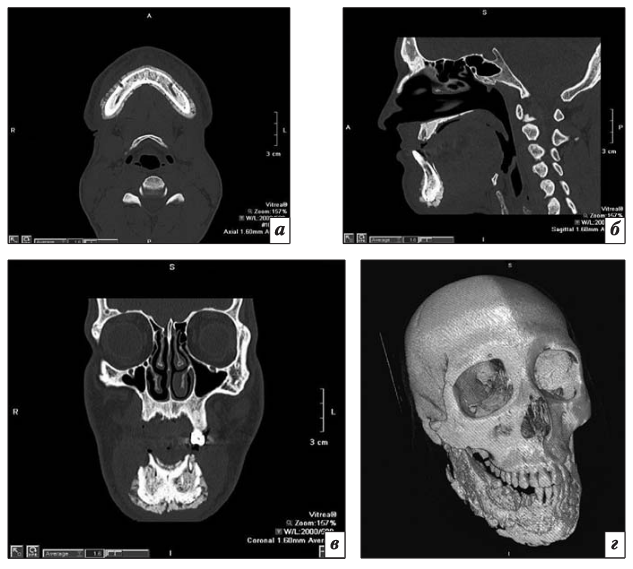
\includegraphics[width=\textwidth]{mskt1}
		\caption{Результаты МСКТ: аксиальная (а), сагиттальная(б), корональная реконструкции и 3D-реконструкция(г). Определяются муфтообразные бахромчатые периостальные наслоения тела и углов нижней челюсти ~\cite{80-157-1-SM}. }
		\label{fig:mskt1}
	\end{figure}

 Ниже выявляется с помощью МСКТ обширный очаг деструкции нижней челюсти без четких и ровных контуров. В области очага деструкции определяются признаки секвестрации костной ткани. В области отростков, ветвей, угла и тела нижней челюсти (преимущественно справа) визуализируются выраженные периостальные наслоения слоистого типа.
 
 	\begin{figure}[H]
 	\centering
 	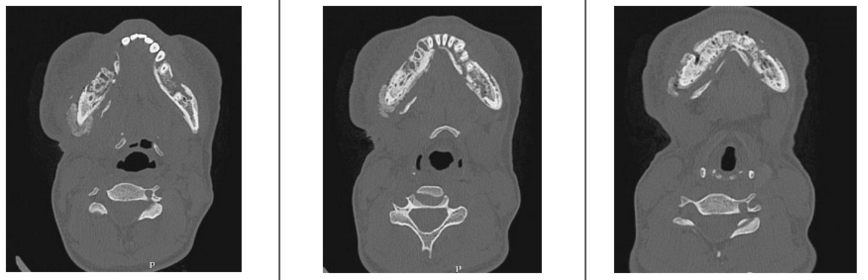
\includegraphics[width=\textwidth]{mskt2}
 	\caption{МСКТ аксиальная реконструкция ~\cite{rejr}. }
 	\label{fig:mskt2}
	 \end{figure}

 	\begin{figure}[H]
	\centering
	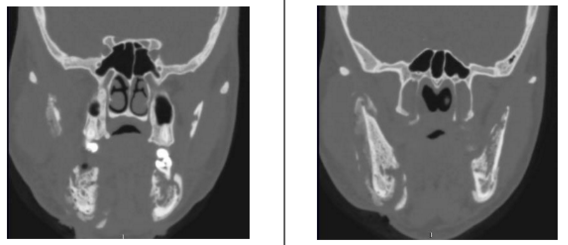
\includegraphics[width=\textwidth]{mskt3}
	\caption{МСКТ коронарная реконструкция ~\cite{rejr}. }
	\label{fig:mskt3}
	\end{figure} 

 	\begin{figure}[H]
	\centering
	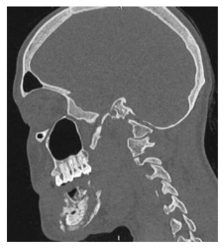
\includegraphics[]{mskt4}
	\caption{МСКТ сагиттальная реконструкция ~\cite{rejr}. }
	\label{fig:mskt4}
	\end{figure} 

 	\begin{figure}[H]
	\centering
	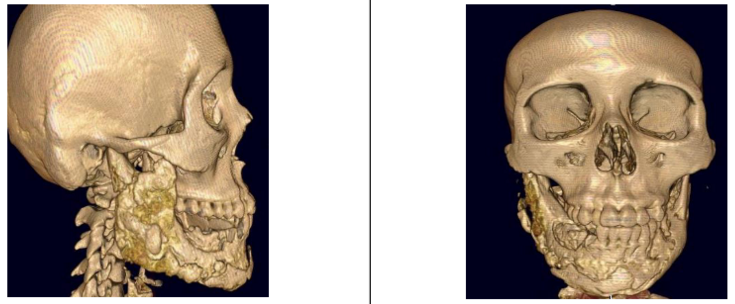
\includegraphics[width=\textwidth]{mskt5}
	\caption{МСКТ 3D реконструкции ~\cite{rejr}. }
	\label{fig:mskt5}
	\end{figure} 

	Данные компьютерной томографии, приведенные ниже, были собраны на на мультиспиральном компьютерном рентгеновском томографе «Somatom Sensation» Siemens.
	
\begin{figure}[H]
	\centering
	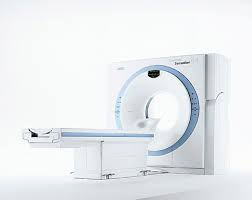
\includegraphics[width=\textwidth]{mskt6}
	\caption{Внешний вид «Somatom Sensation» Siemens. }
	\label{fig:mskt6}
\end{figure} 


	\section{ КЛКТ - конусно-лучевая компьютерная томография}
	Данный вид исследования	выполнялся на аппарате «Galileos» (Sirona) с коническим лучом рентгеновского излучения, со
	специальным режимом FaceScan, при позиционировании пациентов стоя или сидя, в соответствии с лазерными метками. Постпроцессорная	обработка полученных данных включала в себя	построение мультипланарных  реконструкций, также получение изображений в режиме FaceScan. Параметры и критерии оценки, анализируемые при выполнении КЛКТ на всех диагностических этапах, были аналогичны таковым при проведении МСКТ. 
	
	\begin{figure}[H]
	\centering
	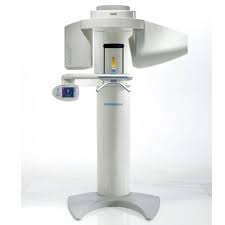
\includegraphics[width=\textwidth]{klkt3}
	\caption{ КЛКТ аппарат «Galileos» (Sirona) ~\cite{rejr} }
	\label{fig:klkt3}
	\end{figure} 

	\begin{figure}[H]
	\centering
	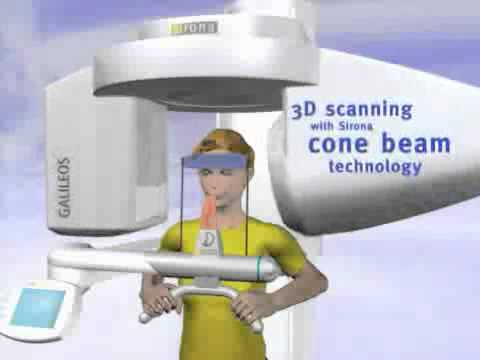
\includegraphics[width=\textwidth]{klkt4}
	\caption{ КЛКТ аппарат «Galileos» (Sirona) ~\cite{rejr} }
	\label{fig:klkt3}
	\end{figure} 
	
	
	Ниже на снимках продемонстрировано как с помощью КЛКТ определяется очаг деструкции альвеолярного отростка верхней челюсти. Неполная вторичная адентия: отсутствуют зубы 1.8-2.8, 3.4-3.8, 4.3-4.8. 
	
	\begin{figure}[H]
		\centering
		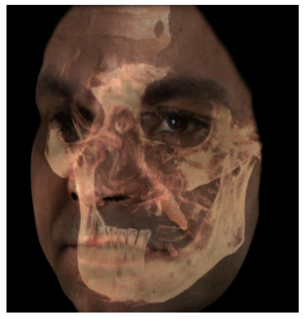
\includegraphics[width=\textwidth]{klkt1}
		\caption{ КЛКТ. 3D-реконструкция в режиме FaceScan ~\cite{rejr} }
		\label{fig:klkt1}
	\end{figure} 
	
		\begin{figure}[H]
		\centering
		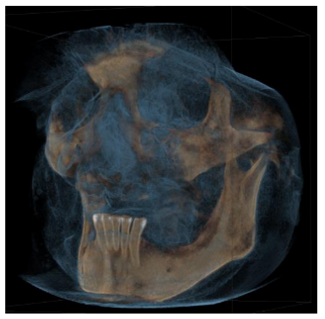
\includegraphics[width=\textwidth]{klkt2}
		\caption{ КЛКТ.  3D-реконструкция с наложением мягких тканей ~\cite{rejr} }
		\label{fig:klkt1}
	\end{figure} 
	
	
	
	\section{ Остеосцинтиграфия}
	Ряд пациентов данной группы предъявлял	жалобы на боли, дисфункцию, отеки со стороны 
	локтевых, тазобедренных, коленных суставов. 
	
	19 пациентам (22 \%) проведена остеосцинтиграфия на гамма-камере (General Electric) с 
	применением радиофармпрепарата (РФП) 99mTc-пирфотеха по стандартной методике 
	(сканирование проведено до уровня коленных 	суставов).  
	
	\begin{figure}[H]
		\centering
		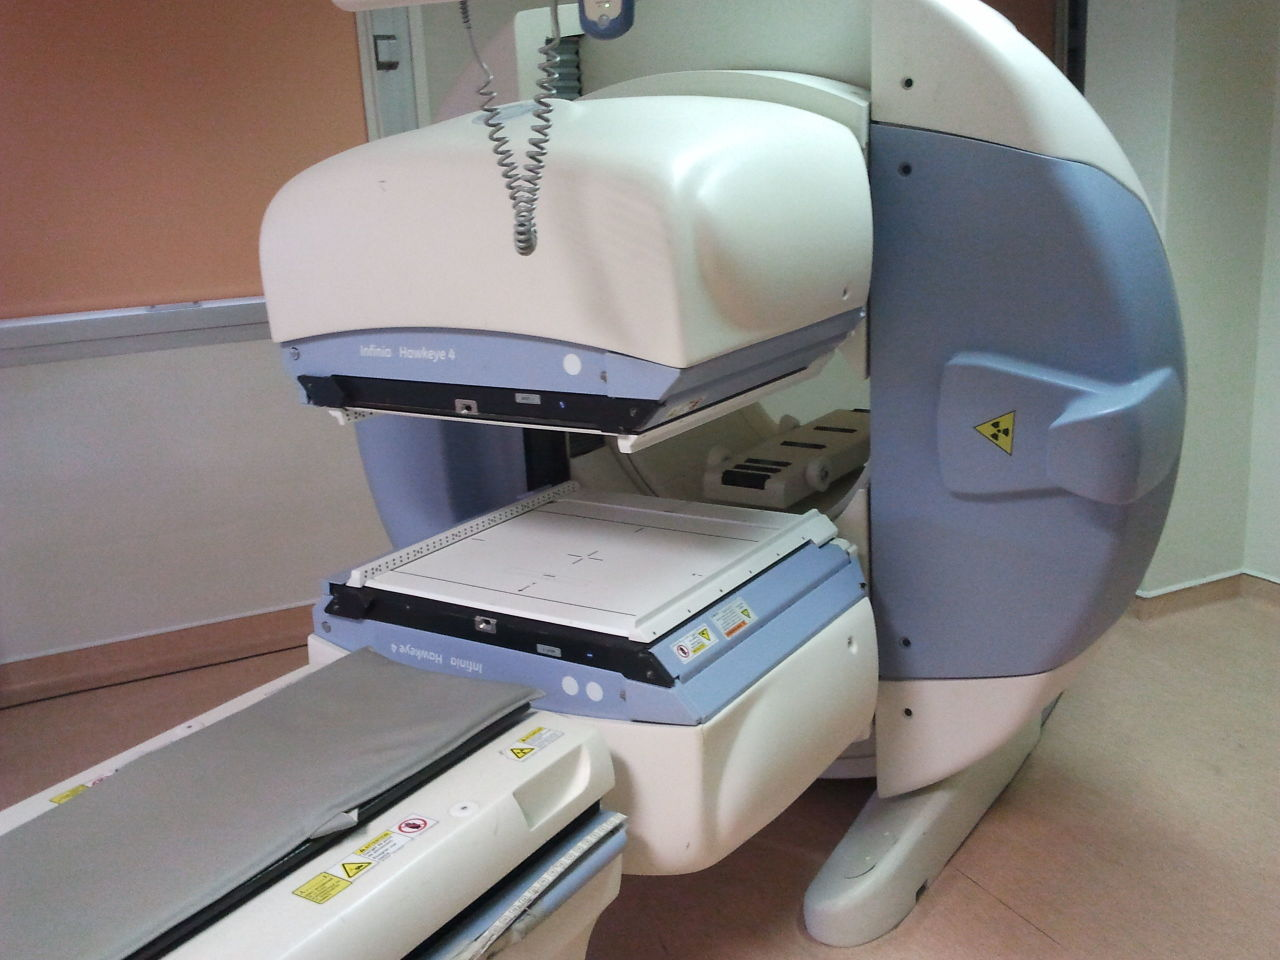
\includegraphics[width=\textwidth]{gk}
		\caption{ Двухдетекторная гамма-камера « Infinia » со встроенным рентгеновским компьютерным томографом «Hawkeye» фирмы «General Electric» }
		\label{fig:gk}
	\end{figure} 

	\begin{figure}[H]
	\centering
	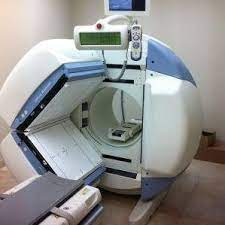
\includegraphics[width=\textwidth]{gk1}
	\caption{ Двухдетекторная гамма-камера « Infinia » со встроенным рентгеновским компьютерным томографом «Hawkeye» фирмы «General Electric» }
	\label{fig:gk1}
	\end{figure} 

	\begin{figure}[H]
	\centering
	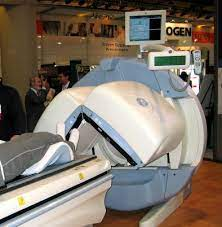
\includegraphics[width=\textwidth]{gk2}
	\caption{ Двухдетекторная гамма-камера « Infinia » со встроенным рентгеновским компьютерным томографом «Hawkeye» фирмы «General Electric» }
	\label{fig:gk2}
	\end{figure} 
	
	С помощью остеосцинтиграммы определяются зоны повешенного накопления РФП в проекции тела верхней челюсти и скуло-глазничного комплекса справа, костей носа, также накопление индикатора отмечается в области правого коленного сустава, рукоятки и тела грудины. 
	
	\begin{figure}[H]
		\centering
		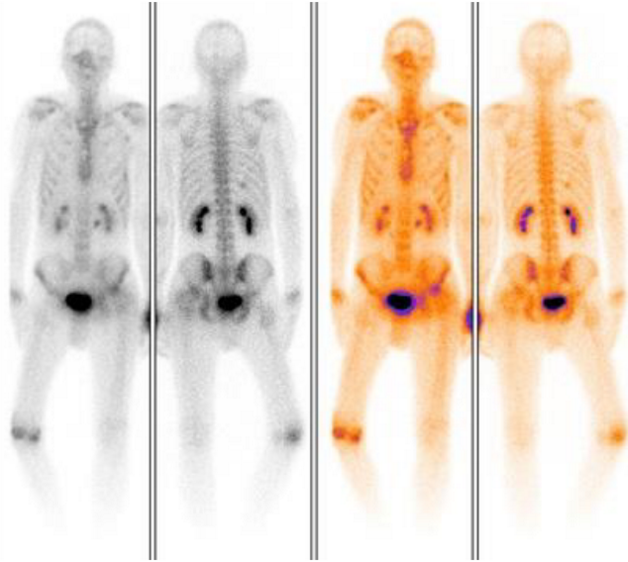
\includegraphics[width=\textwidth]{gk3}
		\caption{ Остеосцинтиграмма ~\cite{rejr} }
		\label{fig:gk3}
	\end{figure} 

	Таким образом, в представленном исследовании пациентам с остеонекрозами на фоне дезоморфиновой зависимости был применен весь спектр лучевых методов на соответствую	щих этапах диагностики и лечения. 

	
	\section{Выводы}
	 Применение полного спектра лучевых методов диагностики (МСКТ,	КЛКТ, радионуклидная диагностика) у дезоморфинзависимых пациентов на всех этапах лечения позволяет полноценно и своевременно установить характер и распространенность патологического процесса, также спланировать тактику дальнейшего хирургического лечения у данных пациентов ~\cite{rejr}. 
	
	\section{Заключение}
	В практической работе были рассмотрены основные методы лучевой диагностики, изучены результаты применения этих методов и проведен анализ эффективности применения методов на примере комплексной лучевой диагностики остеонекрозов у дезоморфинзависимых пациентов.
	
	\begin{thebibliography}{3}
		\bibitem{kataev} Катаев С.С., Зеленина Н.Б., Шилова Е.А. Определение	дезоморфина в моче. Проблемы экспертизы в медицине.	2007; 1: 32-36 

		\bibitem{babkova} Babkova A.A., Serova N.S., Zhivoglyadov D.I., Kureshova D.N., Basin E.M., Pasha S.P. Modern radiological diagnosis of osteonecrosis of the bones of the facial skull in patients with drug dependence. REJR. 2015; 5 (2) suppl.: 178-179 (in Rus	sian).  
		
		\bibitem{basin} Basin E.M., Medvedev Yu.A. Phosphorus necrosis of the jaws. Doctor. 2012; 1: 21-25 (in Russian). 
		
		\bibitem{rsj} Медведев Ю.А., Басин Е.М., Серова Н.С., Коршунова А.В., Бабкова А.А., Курешова Д.Н. Тотальные некрозы костей лицевого черепа у лиц с наркотической зависимостью. Российский стоматологический журнал. 2016; 20 (4): 183-189. DOI 10.18821/1728-2802 2016; 20 (4):183-189
		
		\bibitem{rejr} Серова Н.С., Бабкова А.А., Курешова Д.Н., Паша С.П., Басин Е.М. КОМПЛЕКСНАЯ ЛУЧЕВАЯ ДИАГНОСТИКА ОСТЕОНЕКРОЗОВ У ДЕЗОМОРФИНЗАВИСИМЫХ ПАЦИЕНТОВ. Российский Электронный Журнал Лучевой Диагностики. 2015; 5 (4): 13-23. DOI 10.18821/1728-2802 2016; 20 (4):183-189
			
		\bibitem{rsj_1}   Дерябин  Е.И.,  Миронова  Ю.С.  Клинико-морфологическая  характеристика  остеомиелита  челюстей  у  наркотически  зависи-мых  пациентов.  В  кн.: Материалы  Республиканской  научно-практической конференции с международным участием «Современные достижения и перспективы развития хирургической стоматологии и челюстно-лицевой хирургии». 2010: 23–4.
		
		\bibitem{rsj_2}   Егорова Е.А., Зорина И.С., Сангаева Л.М. Лучевая дифференциальная диагностика остеомиелитов челюстно-лицевой области при  иммунодефицитных  состояниях. Сибирский  медицинский журнал. 2010; 25 (3, Выпуск 2): 31–7.
		
		\bibitem{rsj_3}   Лесовая И.Г., Хименко В.М., Хименко В.В. Клинический опыт оказания специализированной помощи больным с нетипичным течением одонтогенного остеомиелита страдающих наркоманией и синдромом приобретенного иммунодефицита. В кн.: Мате-риалы Всеукраинской научно-практической конференции «Но-вые технологии в стоматологии и челюстно-лицевой хирургии». Харьков;2006: 77–82.
		
		\bibitem{rsj_4}   Маланчук В.А., Бродецкий И.С. Комплексное лечение больных остеомиелитом челюстей на фоне наркотической зависимости. Вестник Витебского государственного медицинского университета. 2014; 13 (2): 115–23.
		
		\bibitem{rsj_5}   Маланчук  В.А.,  Бродецкий  И.С.,  Забудская  Л.Р.  Особенности рентгенологической картины остеомиелита челюстей у больных на фоне наркотической зависимости. Укр. мед. часопис. 2009; 2 (70): 122–5.
		
		\bibitem{rsj_6}   Маланчук В.О., Бродецкий И.С. Комплексное лечение больных остеомиелитом челюстей на фоне наркотической зависимости. В кн.: Материалы Республиканской научно-практической конференции с международным участием «Современные достижения и перспективы развития хирургической стоматологии и челюстно-лицевой хирургии». 2010: 51–3.
		
		\bibitem{rsj_7}   Нестеров  А.П.,  Нестеров  А.А.,  Востриков  И.Н.  Рентгено-диагностика одонтогенного остеомиелита челюстей у лиц с наркотической зависимостью от дезоморфина. Дентал Юг. 2012; 104 (8): 40–2.
		
		\bibitem{rsj_8}   Нестеров А.П., Нестеров А.А., Хабибов Я.Т. Патогенез одонтогенного остеомиелита челюстей у лиц с зависимостью от дезоморфина. Дентал Юг. 2012; 102 (6): 42–4.
		
		\bibitem{rsj_9}    Погосян Ю.М., Акопян К.А. Гаспарян Л.Л. Рентгенодиагностика остеонекроза челюстей у больных, употребляющих наркотическое средство «Крокодил». Вопросы теоретической и клинической медицины. 2013; 16 (2): 44–7.
		
		\bibitem{rsj_10}    Погосян Ю.М., Акопян К.А. Лечение остеонекроза челюстей у больных, употребляющих самодельно изготовленные наркотические средства. Вопросы теоретической и клинической медицины. 2013; 16 (1) 77: 48–51.
		
		\bibitem{rsj_11}    Саберов Р.З., Дробышев А.Ю. Особенности хирургического лечения остеонекроза челюстей на фоне наркотической зависимости. Стоматология для всех. 2013; (3): 26–33.
		
		\bibitem{rsj_12}    Столбова М.В., Пугаева М.О., Боркина А.Н., Нигматулина Э.Ф., Рыжкова О.В. Особенности внебольничной пневмонии у дезоморфиновых и полинаркоманов с вичинфекцией. Вестник ОГУ. 2011; 131 (12): 303–6.
		
		\bibitem{rsj_13}    Тимофеев А.А., Дакал А.В. Особенности клинического течения и  хирургического  лечения  первичных  одонтогенных  воспалительных очагов у больных с гнойно-воспалительными заболеваниями мягких тканей, употреблявших наркотик «Винт». Со-временная cтоматология. 2010; (3): 123–7.
		
		\bibitem{rsj_14}    Тимофеев  А.А.,  Дакал  А.В.  Применение  иммунокоррегирующей терапии в комплексном лечении наркозависимых больных с одонтогенными гнойно-воспалительными заболеваниями мягких тканей. Современная стоматология. 2009; (2): 85–8.
		
		\bibitem{rsj_15}    Уракова Е.В., Нестеров О.В. Выбор методов оперативного лечения больных с дезоморфиновым остеомиелитом. Практическая медицина. 2014; 80 (4) 2: 142–4.	
		
		\bibitem{80-157-1-SM} Серова Н.С., Курешова Д.Н., Бабкова А.А., Басин Е.М. Многосрезовая компьютерная томография в диагностике токсических фосфорных некрозов челюстей. Вестник рентгенологии и радиологии. 2015;(5):11-16. https://doi.org/10.20862/0042-4676-2015-0-5-42-49
		
		\bibitem{op100}GE Healthcare Orthopantomograph® OP100 D Orthoceph® OC100 D User \& Technical Manual
		
		\bibitem{st} Basin EM, Medvedev YA. [Toxic phosphorus osteonecrosis of facial bones among drug addicts to desomorphine and pervitin. Part I]. Stomatologiia (Mosk). 2015;94(2):53-57. Russian. doi: 10.17116/stomat201594253-57. PMID: 26171547.
			
		\end{thebibliography}

\end{document}	